\documentclass[tikz, border=10pt]{standalone}
\usepackage{amsmath,amssymb}

\begin{document}
	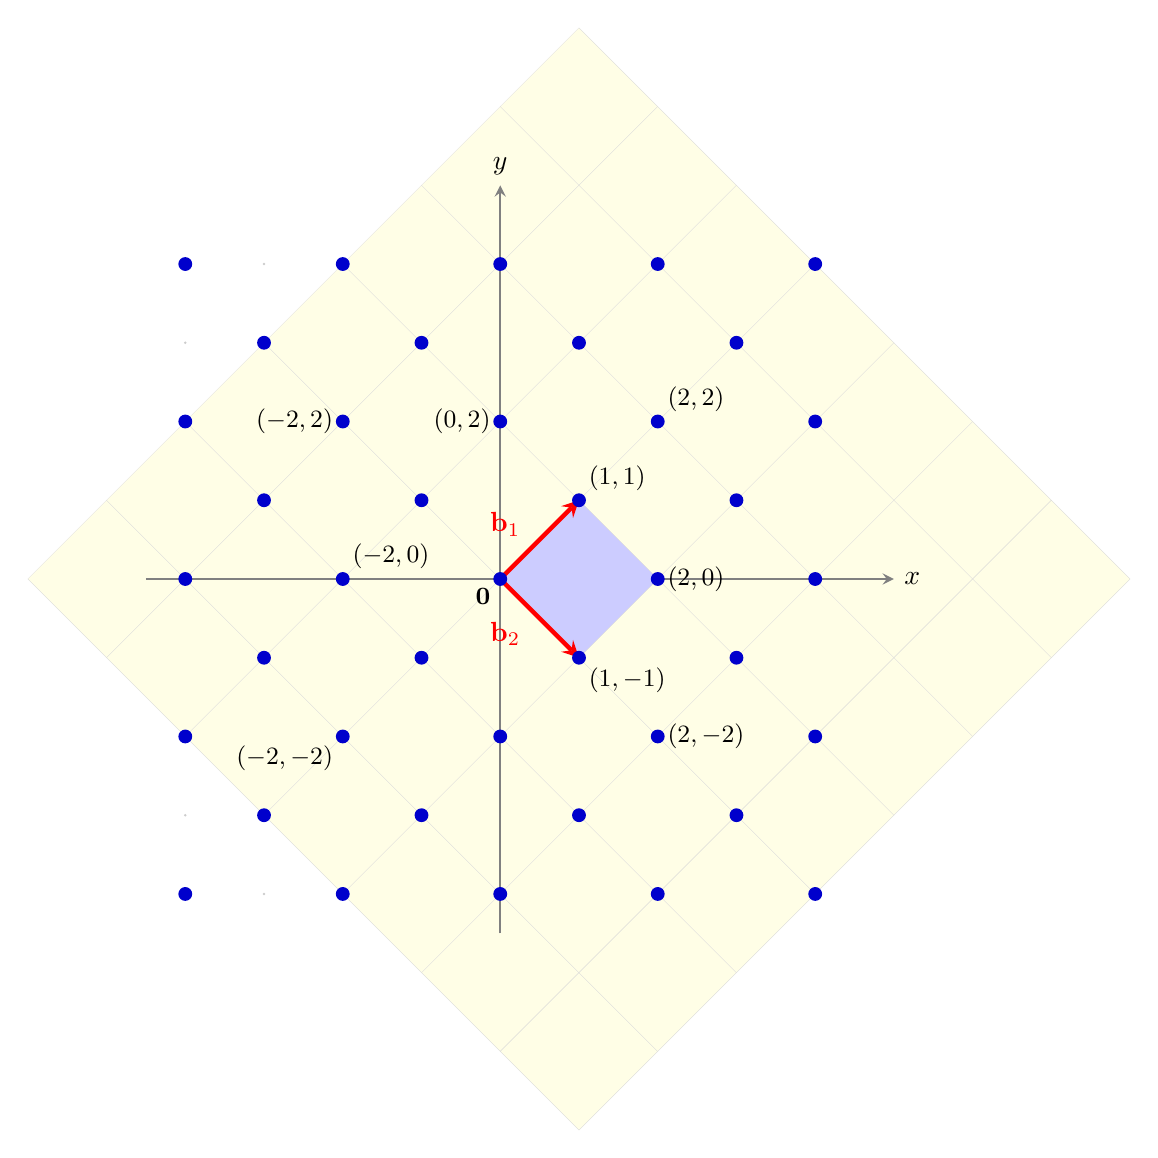
\begin{tikzpicture}[>=stealth]
		
		% Define basis vectors b1, b2 that generate this lattice
		% b1 = (1, 1), b2 = (1, -1)
		\def\bax{1} \def\bay{1}
		\def\bbx{1} \def\bby{-1}
		
		% Define the fundamental domain path (parallelogram spanned by b1, b2)
		% vertices: O, b1, b1+b2=(2,0), b2
		\def\cellpath{(0,0) -- (\bax,\bay) -- ({\bax+\bbx},{\bay+\bby}) -- (\bbx,\bby) -- cycle}
		
		% Range for loops to cover visibility, e.g., -4 to 4
		\def\xmin{-4} \def\xmax{4}
		\def\ymin{-4} \def\ymax{4}
		
		% ==========================================
		% LAYER 1: Background context and Tiling
		% ==========================================
		
		% Draw a light underlying grid of all integer points Z^2 for context
		\foreach \x in {\xmin,...,\xmax} {
			\foreach \y in {\ymin,...,\ymax} {
				\fill[gray!40] (\x, \y) circle (0.5pt);
			}
		}
		
		% Tiling copies of P(B) to visually demonstrate covering.
		% We use i, j indices in [-3, 3] to cover visibility.
		\foreach \i in {-3, -2, -1, 0, 1, 2, 3} {
			\foreach \j in {-3, -2, -1, 0, 1, 2, 3} {
				% Calculate current lattice point y = i*b1 + j*b2
				\coordinate (Lpoint) at ({\i*\bax + \j*\bbx}, {\i*\bay + \j*\bby});
				
				% Shade the translated copy y + P(B).
				% Light yellow fill with subtle gray boundaries creating the tiling.
				\fill[yellow!10!white, draw=gray!30, line width=0.1pt, shift={(Lpoint)}] \cellpath;
			}
		}
		
		% Draw axes, scaled to visibility
		\draw[->, thick, gray] ({\xmin-0.5},0) -- ({\xmax+1},0) node[right, black] {$x$};
		\draw[->, thick, gray] (0,{\ymin-0.5}) -- (0,{\ymax+1}) node[above, black] {$y$};
		
		% ==========================================
		% LAYER 2: Fundamental Domain and Basis
		% ==========================================
		
		% Highlight the primary fundamental domain at the origin with distinctive blue
		\fill[blue!20, draw=gray!30, line width=0.1pt] \cellpath;
		
		% Draw and label the basis vectors b1, b2 from the origin
		\draw[->, ultra thick, red] (0,0) -- (\bax,\bay) node[midway, above left, xshift=-1mm, yshift=-1mm] {$\mathbf{b}_1$};
		\draw[->, ultra thick, red] (0,0) -- (\bbx,\bby) node[midway, below left, xshift=-1mm, yshift=1mm] {$\mathbf{b}_2$};
		
		% Label the fundamental domain P(B)
%		\node[blue!80!black, font=\bfseries] at ({(\bax+\bbx)/2}, {(\bay+\bby)/2}) {$\mathcal{P}(B)$};
		
		% Mark vertices of the fundamental domain
		\fill[black] (0,0) circle (2pt) node[below left] {\small $\mathbf{0}$};
		\fill[black] (\bax,\bay) circle (2pt) node[above right] {\small $(1,1)$};
		\fill[black] ({\bax+\bbx},{\bay+\bby}) circle (2pt) node[right] {\small $(2,0)$};
		\fill[black] (\bbx,\bby) circle (2pt) node[below right] {\small $(1,-1)$};
		
		% ==========================================
		% LAYER 3: Marking All Lattice Points of \Lambda
		% ==========================================
		
		% Draw prominent lattice points in a nested loop with condition check.
		% For each point (x,y), check if x-y is even.
		\foreach \x in {\xmin,...,\xmax} {
			\foreach \y in {\ymin,...,\ymax} {
				% Use pgfmath to check if mod((x-y), 2) is 0.
				% Must use integer values. Use \int{}
				\pgfmathsetmacro{\diff}{\x-\y}
				\pgfmathparse{mod(int(\diff), 2) == 0 ? 1 : 0}
				\ifnum\pgfmathresult=1\relax
				% Point satisfies the condition, plot in blue
				\fill[blue!80!black] (\x, \y) circle (2.5pt);
				% Optionally label key points not on axes and far, e.g., (2,2)
				\ifnum\x=2\relax \ifnum\y=2\relax \node[above right] at (\x,\y) {\small $(2,2)$};\fi\fi
				\ifnum\x=-2\relax \ifnum\y=-2\relax \node[below left] at (\x,\y) {\small $(-2,-2)$};\fi\fi
				\ifnum\x=0\relax \ifnum\y=2\relax \node[left] at (\x,\y) {\small $(0,2)$};\fi\fi
				\ifnum\x=2\relax \ifnum\y=-2\relax \node[right] at (\x,\y) {\small $(2,-2)$};\fi\fi
				\ifnum\x=-2\relax \ifnum\y=2\relax \node[left] at (\x,\y) {\small $(-2,2)$};\fi\fi
				\ifnum\x=-2\relax \ifnum\y=0\relax \node[above right] at (\x,\y) {\small $(-2,0)$};\fi\fi
				\fi
			}
		}
		
%		% ==========================================
%		% LAYER 4: Explanation Text Box
%		% ==========================================
%		\node[align=left, anchor=north west, fill=white, draw=black, inner sep=5pt, font=\small] at ({\xmin-2.5}, {\ymax+2.2}) {
%			\textbf{Checkerboard Lattice $\Lambda$} \\
%			$\Lambda = \{(x,y) \in \mathbb{Z}^2 : x - y \in 2\mathbb{Z}\}$ \\
%			Condition is equivalent to $x \equiv y \pmod 2$. \\
%			Points are (even, even) or (odd, odd). \\
%			Basis used: $\mathbf{b}_1 = \begin{pmatrix} 1 \\ 1 \end{pmatrix}, \ \mathbf{b}_2 = \begin{pmatrix} 1 \\ -1 \end{pmatrix}$ \\
%			Tiled cells demonstrate fundamental domains. \\
%			Large blue dots are lattice points. \\
%			Small gray dots are full $\mathbb{Z}^2$ points.
%		};
		
	\end{tikzpicture}
\end{document}